% How to make codeblock
% \begin{lstlisting} ... \end{lstlisting}


\documentclass[12pt,a4paper,oneside]{report}

% --- Packages ---
\usepackage[utf8]{inputenc}
\usepackage[english]{babel}
\usepackage{graphicx}
\graphicspath{ {./Assets/} }
\usepackage{amsmath, amssymb}
\usepackage[dvipsnames]{xcolor}
\usepackage{booktabs} % For professional tables
\usepackage{hyperref} % For clickable links
\usepackage{listings} % For showing your Python/Mesa code
\usepackage{geometry}
\geometry{left=3cm, right=2.5cm, top=2.5cm, bottom=2.5cm}

% Code snippet styling
\definecolor{codegreen}{rgb}{0,0.6,0}
\lstset{
    commentstyle=\color{codegreen},
    keywordstyle=\color{magenta},
    numberstyle=\tiny,
    stringstyle=\color{purple},
    basicstyle=\ttfamily\small,
    breaklines=true,
    captionpos=b,
    keepspaces=true,
    showspaces=false,
    language=Python
}

% --- Info ---
\title{Temporary title \\
\large \& Subtitle}
\author{Daan Grupping}
\date{\today}

\begin{document}
\maketitle
\begin{abstract}

\end{abstract}

\tableofcontents

% --- Chapters ---

\chapter{Introduction}
\chapter{Exploratory Data Analysis}
\begin{figure}[htbp] % h=here, t=top, b=bottom, p=page
    \centering
    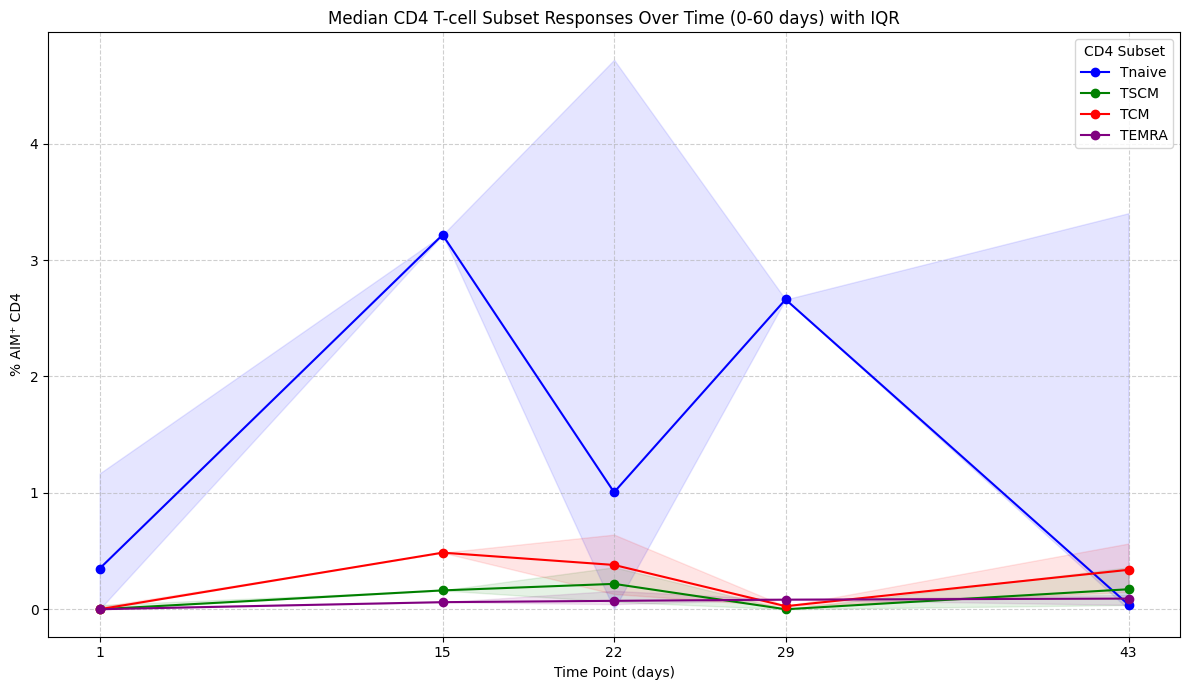
\includegraphics[width=0.8\textwidth]{EDA1} 
    \caption{.}
    \label{fig:}
\end{figure}
\chapter{Hypothesis}
\chapter{Model Design}
\chapter{Implementation}
\chapter{Sanity Checks}
\chapter{Calibration}
\chapter{Validation}
\chapter{Sensitivity}
\chapter{Ablation}
\chapter{Per-Patient}
\chapter{Interpretation}



% --- Bibliography ---
\nocite{*} 
\bibliographystyle{plain}
\bibliography{references}

\appendix
\chapter{Code}

\end{document}